% !TeX spellcheck = sk_SK-Slovak
\chapter*{Úvod} % chapter* je necislovana kapitola
\addcontentsline{toc}{chapter}{Úvod} % rucne pridanie do obsahu
\markboth{Úvod}{Úvod} % vyriesenie hlaviciek

V nemocničnom informačnom systéme Univerzitnej nemocnice v Bratislave nie je možnosť jednoducho získať tabuľku obsahujúcu dáta jedného pacienta respektíve skupiny pacientov, tieto dát sa získavali ručne buď postupným kopírovaním jednotlivých dát nachádzajúcich sa v rôznych častiach informačného systému alebo ich hľadaním a následným prepisovaním z prepúšťacej správy.

Tento proces bolo potrebné opakovať pre každého jedného pacienta čo bolo časovo náročné a vyžadovalo si nezanedbateľné množstvo ľudskej práce.

Hlavným účelom tejto práce je vytvorenie softvéru, ktorý pomôže výrazne zrýchliť a zjednodušiť získavanie týchto dát. Tento softvér na svojom vstupe dostane prepúšťaciu správu pacienta a jeho krvné výsledky v podobe textu ktorý je čiastočne generovaný nemocničným informačným systémom ale z veľkej časti je písaný lekárom a následne z týchto ne-štrukturalizovaných dát získava jednotlivé požadované dáta. Počas získavania dát si zároveň zapamätáva informáciu o dátach ktoré sa buď nájsť nepodarilo alebo sa počas ich získavania objavil nejaký problém ako napríklad viac rôznych hodnôt alebo protirečiace informácie. Výsledkom je asociatívne pole v ktorom sú ako kľúče použité názvy hľadaných informácii a text obsahujúci informáciu o nenájdených a problémových údajoch. 

\begin{figure}
	%vlozenie samotneho obrazku vycentrovaneho a vhodnej velkosti
	%obrazok je v subore images/cervik.png
	\centerline{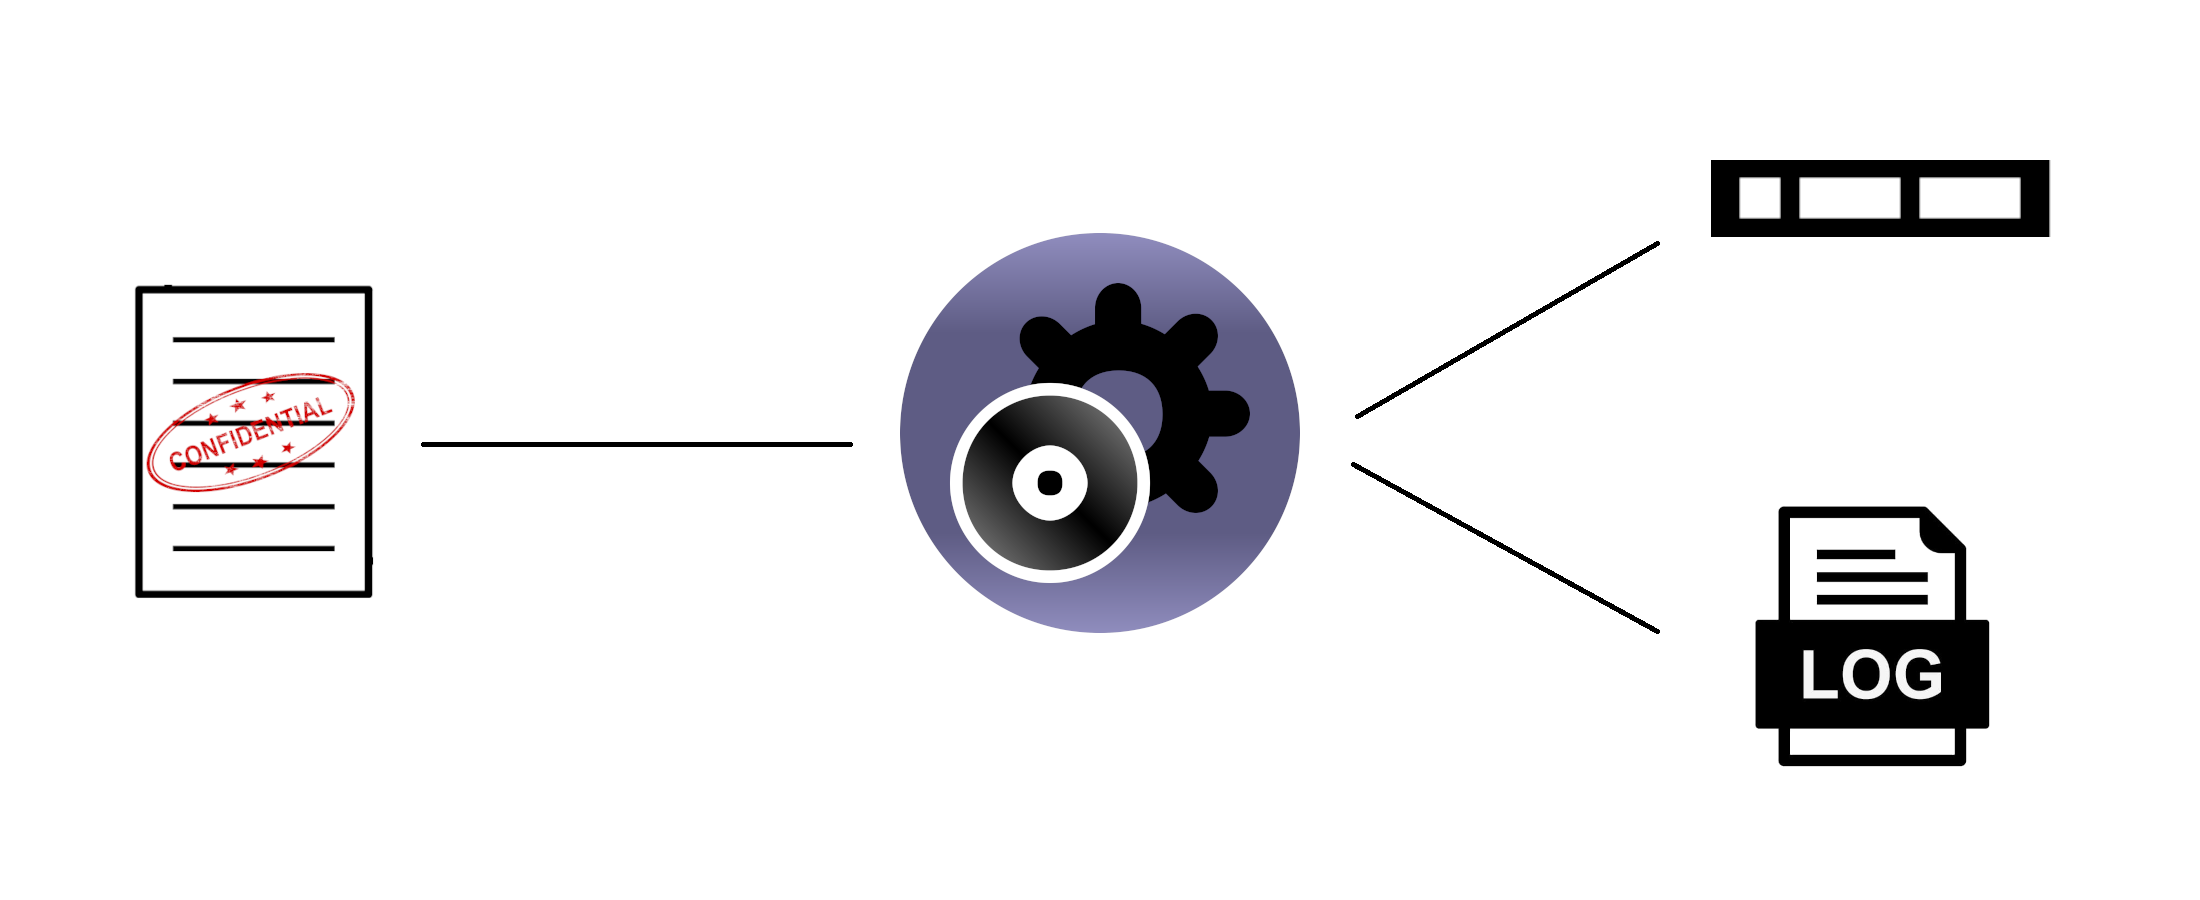
\includegraphics[width=0.8\textwidth]{images/system_jedna_sprava}}
	%popis obrazku
	\caption[Fungovanie systému pre jednu správu]{Fungovanie systému pre jednu správu}
	%id obrazku, pomocou ktoreho sa budeme na obrazok odvolavat
	\label{obr:systemJedna}
\end{figure}
\newpage
Okrem spracovania jedného pacienta je tento systém schopný spracovať aj väčšiu množinu pacientov pričom v takomto prípade už nie je výsledkom asociatívne pole ale je ním tabuľka v ktorej sú získavané údaje stĺpcami a jednotlivý pacienti riadkami. Zároveň informácia o nenájdených a problémových sa zapisuje do logovacieho súboru spolu s informáciou pričom vždy je v súbore zapísané aj o ktorého pacienta ide a ktorom hárku sa nachádza jeho prepúšťacia správa a krvné výsledky.
\begin{figure}
	%vlozenie samotneho obrazku vycentrovaneho a vhodnej velkosti
	%obrazok je v subore images/cervik.png
	\centerline{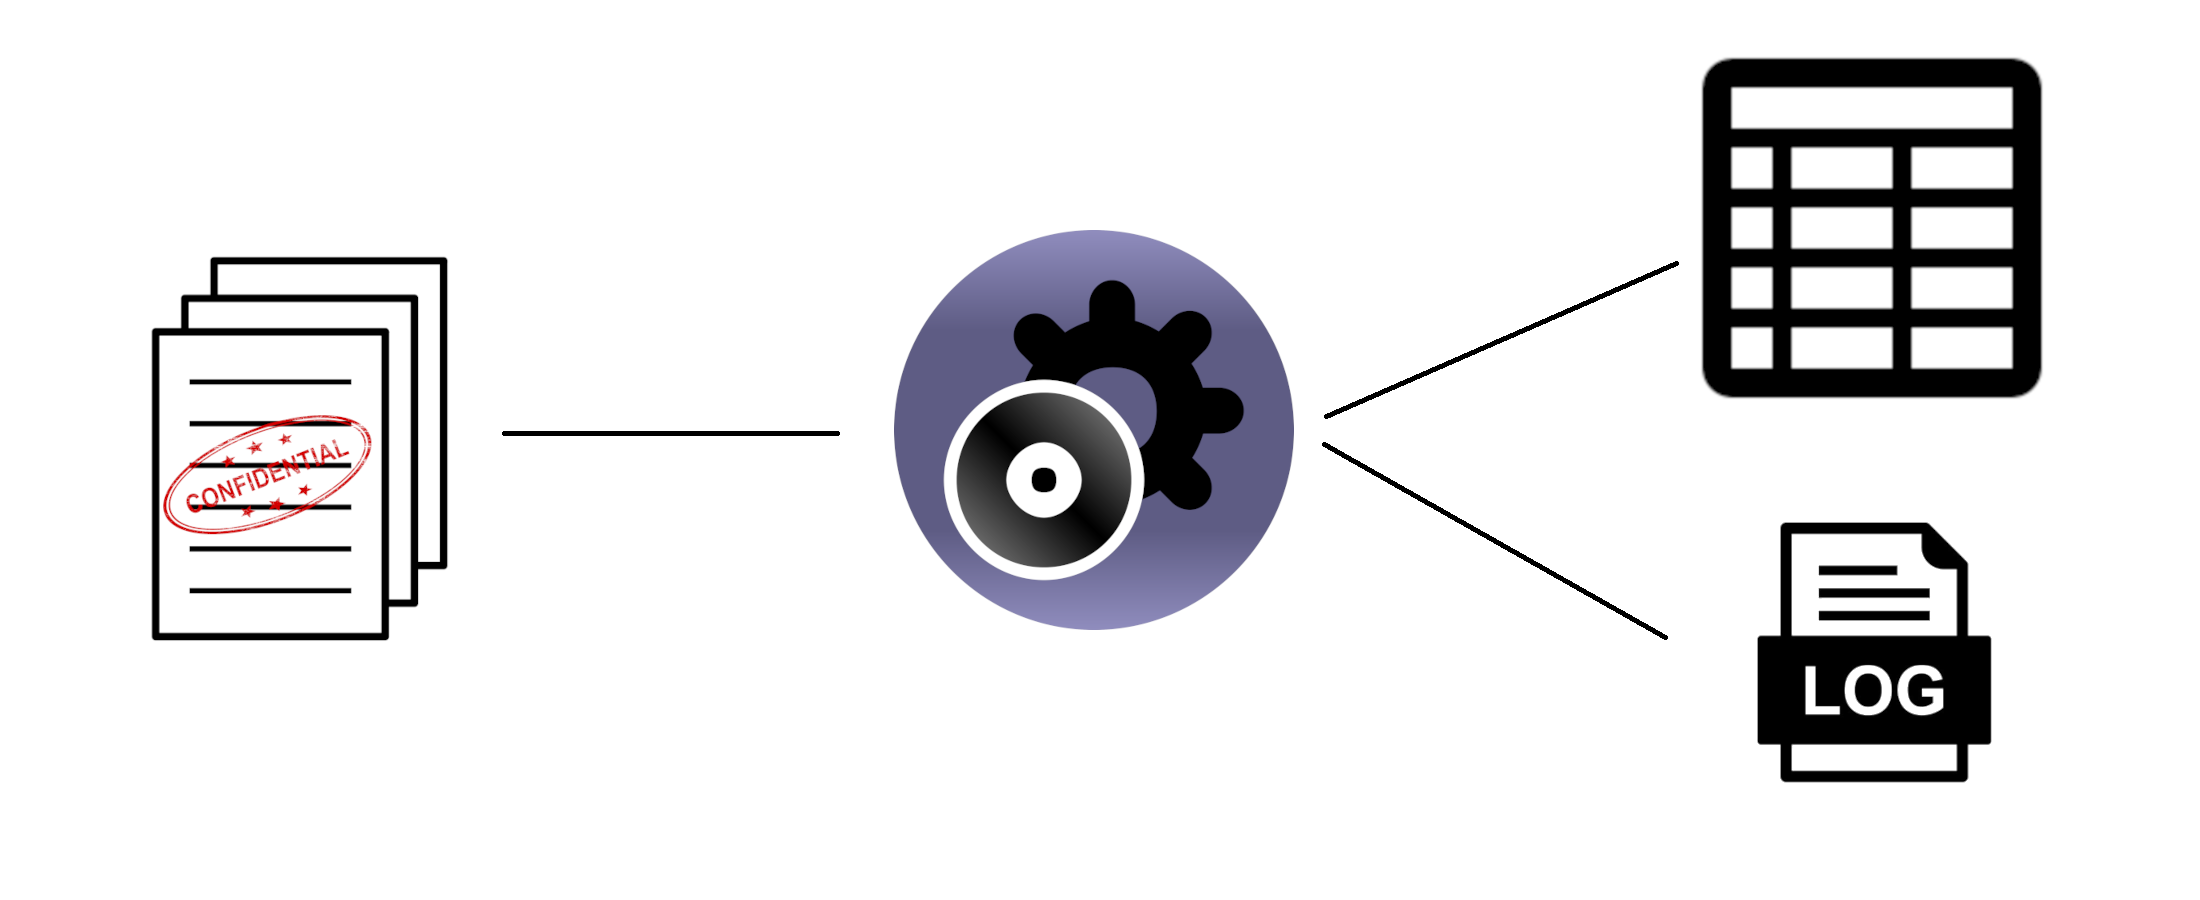
\includegraphics[width=0.8\textwidth]{images/system_viac_sprav}}
	%popis obrazku
	\caption[Fungovanie systému pre množinu správ]{Fungovanie systému pre množinu správ}
	%id obrazku, pomocou ktoreho sa budeme na obrazok odvolavat
	\label{obr:systemJedna}
\end{figure}

Práca je rozdelená do piatich kapitol. V prvá obsahuje informácie o podobných softvéroch. Druhá kapitola sa zameriava na štruktúru prepúšťacej správy a dáta ktoré sa z nej snažíme získať. Tretia kapitola obsahuje problémy ktoré sa objavili pre jednotlivé získavané informácie a aké spôsoby riešenia sme sa rozhodli použiť. V štvrtej je analýza chybovosti softvéru. Posledná kapitola je o modifikáciách softvéru aby bol jednoduchšie použiteľný a modifikovateľný pre iné podobné použitia.

%\begin{quote}
%Úvod je prvou komplexnou informáciou o práci, jej cieli, obsahu a štruktúre. Úvod sa 
%vzťahuje na spracovanú tému konkrétne, obsahuje stručný a výstižný opis 
%problematiky, charakterizuje stav poznania alebo praxe v oblasti, ktorá je predmetom 
%školského diela a oboznamuje s významom, cieľmi a zámermi školského diela. Autor 
%v úvode zdôrazňuje, prečo je práca dôležitá a prečo sa rozhodol spracovať danú tému. 
%Úvod ako názov kapitoly sa nečísluje a jeho rozsah je spravidla 1 až 2 strany.
%\end{quote}


